\documentclass[12pt, a4paper]{article}
\usepackage[utf8]{inputenc}
\usepackage[english]{babel}
\usepackage{amsmath}
\usepackage{csquotes}
\usepackage{mathtools}
\usepackage{graphicx}
\usepackage{geometry}
\usepackage{setspace}
\usepackage{longtable}
\usepackage{float}
\usepackage[colorlinks=true, allcolors=blue]{hyperref}

\usepackage[style=authoryear]{biblatex}
\addbibresource{Bibliography.bib}

\geometry{top = 2.5cm, bottom = 2.5cm, left= 3cm, right= 3cm}

\title{The Compound Pendulum B}
\author{Lee Farrugia \\ Experiment 10 \\ Group 1A}

\date{$8^{\text{th}}$ November 2021}

\begin{document}

\maketitle

\section*{Aim}
The aim of this experiment is to find the gravitational constant with the use of a non-uniform pendulum, with unkown masses. 

\section*{Diagram}
\begin{figure}[H]
    \centering
    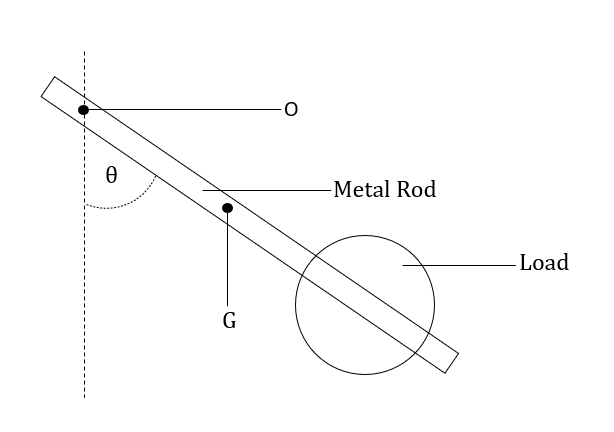
\includegraphics[width=\textwidth]{Experiment 10 Diagram.png}
    \caption{Apparatus Setup}
    \label{fig:set up}
\end{figure}

\section*{List of Apparatus}
Metal rod with unknown mass m, a load with unknown mass M, two types of pivots, a stopwatch, meter ruler, chalk.

\section*{Procedure}
\begin{enumerate}
    \item The length of the metal rod was measured and denoted as \textit{L}.
    \item The metal rod was balanced using a pivot and the center of gravity called G was then marked with a piece of chalk.
    \item The load was then placed a certain distance away from G and the rod was re-balanced. The new center of gravity was then marked with chalk and the distance from G to the new point was measured and called \textit{x}, and the distance from the new point to the center of the load was measured and called \textit{y}. Repeated readings at different positions were taken. This was repeated for a total of 5 different positions of the load.
    \item A graph of $x$ vs $y$ was then plotted.
    \item The apparatus was then set up as shown in the diagram with the load about 5 cm away from G. The distance between G and the pivot point O was called distance \textit{h}, and the distance from the load to O was called \textit{l}. The periodic time \textit{T} for small oscillations of the loaded rod was determined. This was repeated for a total of 5 different values of \textit{l} which was increased by 5 cm each time.
    \item A graph of $T^2$ vs $l_0$ was then plotted. 
\end{enumerate}

\section*{Precautions}
\begin{itemize}
    \item[-] It was made sure that the oscillations done by the pendulum were of a small angle.
    \item[-] The pendulum was allowed to oscillate freely before the timer was started.
    \item[-] If the pendulum started to gyrate it was stopped and restarted with a smaller angle.
    \item[-] The time for 20 oscillations was found and then divided by 20 in order to determine the periodic time.
    \item[-] The oscillations were timed from a position such that it was at the maximum amplitude of the oscillation.
\end{itemize}

\section*{Sources of Error}
\begin{itemize}
    \item[-] Parallax error when reading from the meter ruler to the point on the rod when measuring \textit{y} as the load prohibited direct contact to the rod. 
    \item[-] The open windows, students' movements may have created wind currents which made the pendulum gyrate.
    \item[-] The metal rod was not uniform as it was slightly damaged on one end thus affecting the center of gravity.
    \item[-] The pivot used in order to balance the rod was thinner than the minimum readability of the meter ruler thus it may have affected the determination of the center of gravity.
    \item[-] The pivot used to find the center of gravity was not very thin to be considered as negligible, this may also have affected the position of the center of gravity.
    \item[-] It was possible that the number of 20 oscillations was miscounted and thus obtaining a value for more or less than 20 oscillations, thus, affected the periodic time.
    \item[-] Human reaction time will have affected the readings taken for the periodic time of the oscillations.
\end{itemize}

\section*{Data and Graphs}

\begin{table}[H]
\centering
\caption{Length of rod}\label{tab: Table 1}
\medskip
    \begin{tabular}{| c |}
        \hline \text{$L {\textmd{/m}}$}\\
        \hline \text{\textpm 0.01}\\
        \hline
         1.214\\
         1.215\\
         1.215\\
        \hline
    \end{tabular}
\end{table}

\begin{center}
\begin{longtable}{| c | c | c | c | c | c | c | c | c | c | c |}
\caption{x and y distances} \label{tab:Table 2}\\
    \hline \text{$x_1 {\textmd{/m}}$} & \text{$y_1 {\textmd{/m}}$} & \text{$x_2 {\textmd{/m}}$} & \textbf{$y_2 {\textmd{/m}}$} & \text{$x_3 {\textmd{/m}}$} & \textbf{$y_3 {\textmd{/m}}$} & \text{$x_4 {\textmd{/m}}$} & \textbf{$y_4 {\textmd{/m}}$} & \text{$x_5 {\textmd{/m}}$} & \textbf{$y_5 {\textmd{/m}}$}\\ \hline 
    
    \hline \text{\textpm\ 0.01} & \text{\textpm\ 0.01} & \text{\textpm\ 0.01} & \text{\textpm\ 0.01} & \text{\textpm\ 0.01} & \text{\textpm\ 0.01} & \text{\textpm\ 0.01} & \text{\textpm\ 0.01} & \text{\textpm\ 0.01} & \text{\textpm\ 0.01}\\ \hline 
    \endfirsthead
    
    \hline \text{$x_1 {\textmd{/m}}$} & \text{$y_1 {\textmd{/m}}$} & \text{$x_2 {\textmd{/m}}$} & \textbf{$y_2 {\textmd{/m}}$} & \text{$x_3 {\textmd{/m}}$} & \textbf{$y_3 {\textmd{/m}}$} & \text{$x_4 {\textmd{/m}}$} & \textbf{$y_4 {\textmd{/m}}$} & \text{$x_5 {\textmd{/m}}$} & \textbf{$y_5 {\textmd{/m}}$}\\ \hline  

    \hline \text{\textpm\ 0.01} & \text{\textpm\ 0.01} & \text{\textpm\ 0.01} & \text{\textpm\ 0.01} & \text{\textpm\ 0.01} & \text{\textpm\ 0.01} & \text{\textpm\ 0.01} & \text{\textpm\ 0.01} & \text{\textpm\ 0.01} & \text{\textpm\ 0.01} \\ \hline  
    \endhead

    \hline
    \endfoot

0.061 & 0.047 & 0.107 & 0.076 & 0.174 & 0.115 & 0.222 & 0.147 & 0.290 & 0.185 \\
0.064 & 0.055 & 0.109 & 0.075 & 0.175 & 0.114 & 0.223 & 0.146 & 0.291 & 0.184 \\
0.063 & 0.051 & 0.108 & 0.076 & 0.173 & 0.113 & 0.224 & 0.147 & 0.293 & 0.187
\end{longtable}
\end{center}

\begin{center}
\begin{longtable}{| c | c | c | c | c | c | c |}
\caption{h distance, l distance and Time} \label{tab:Table 3}\\
    \hline \text{$h {\textmd{/m}}$} & \text{$l {\textmd{/m}}$} & \text{$t_1 {\textmd{/s}}$} & \text{$t_2 {\textmd{/s}}$} & \textbf{$t_3 {\textmd{/s}}$} & \text{$T_{avg} {\textmd{/s}}$} & \textbf{$T^2 /s^2$}\\ \hline  
    
    \hline \text{\textpm\ 0.01} & \text{\textpm\ 0.01} & \text{\textpm\ 0.3} & \text{\textpm\ 0.3} & \text{\textpm\ 0.3} & &\\ \hline
    \endfirsthead
    
    \hline \text{$h {\textmd{/m}}$} & \text{$l {\textmd{/m}}$} & \text{$t_1 {\textmd{/s}}$} & \text{$t_2 {\textmd{/s}}$} & \textbf{$t_3 {\textmd{/s}}$} & \text{$T_{avg} {\textmd{/s}}$} & \textbf{$T^2 /s^2$}\\ \hline  
    
    \hline \text{\textpm\ 0.01} & \text{\textpm\ 0.01} & \text{\textpm\ 0.3} & \text{\textpm\ 0.3} & \text{\textpm\ 0.3} & &\\ \hline
    \endhead
    
    \hline
    \endfoot
    
21.60  & 0.05 & 26.3 & 26.3 & 26.4 & 1.3172 & 1.734928028 \\
21.50 & 0.10 & 26.7 & 26.7 & 26.7 & 1.3332 & 1.777333361 \\
21.60  & 0.15 & 27.0 & 27.2 & 27.1  & 1.3553 & 1.836928444 \\
      & 0.20 & 28.0 & 28.2 & 28.3 & 1.4072 & 1.980118028 \\
      & 0.25 & 29.2 & 28.9  & 29.1 & 1.4518 & 2.107820028        
\end{longtable}
\end{center}

\begin{figure}
    \centering
    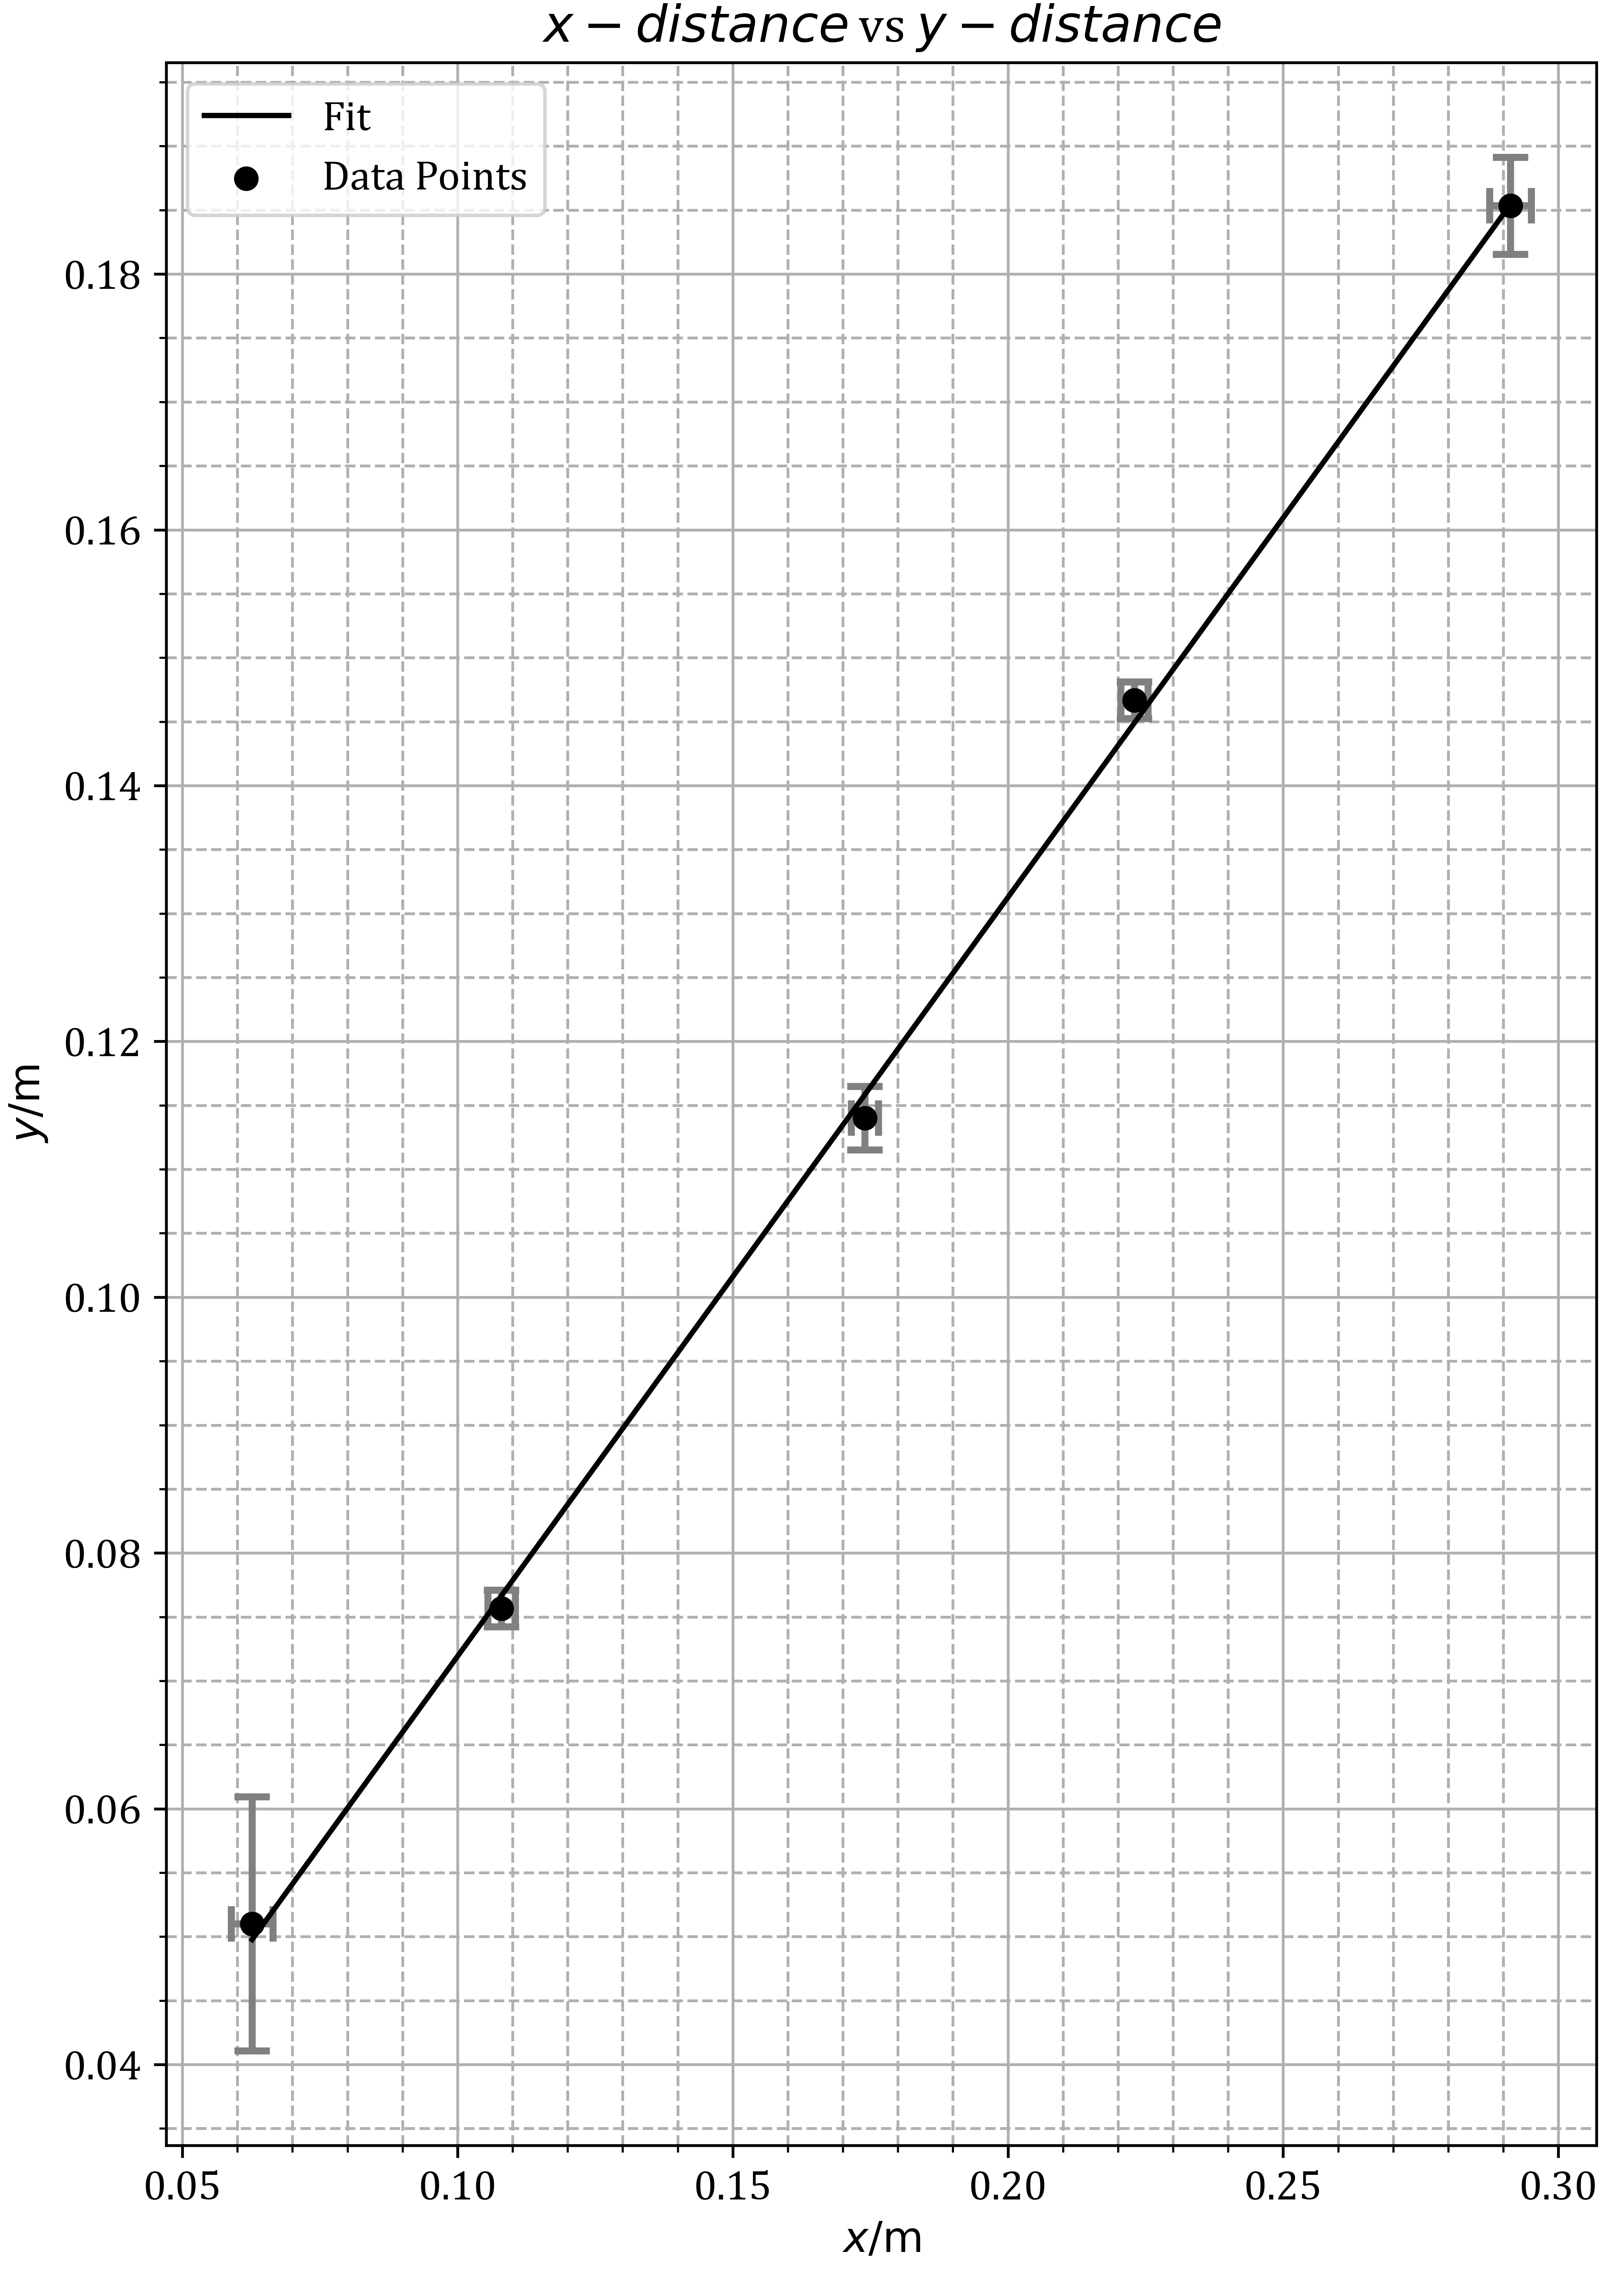
\includegraphics[width=\textwidth]{mMgraph.png}
    \caption{x-distance vs y-distance}
    \label{fig:m/M graph}
\end{figure}

\begin{figure}
    \centering
    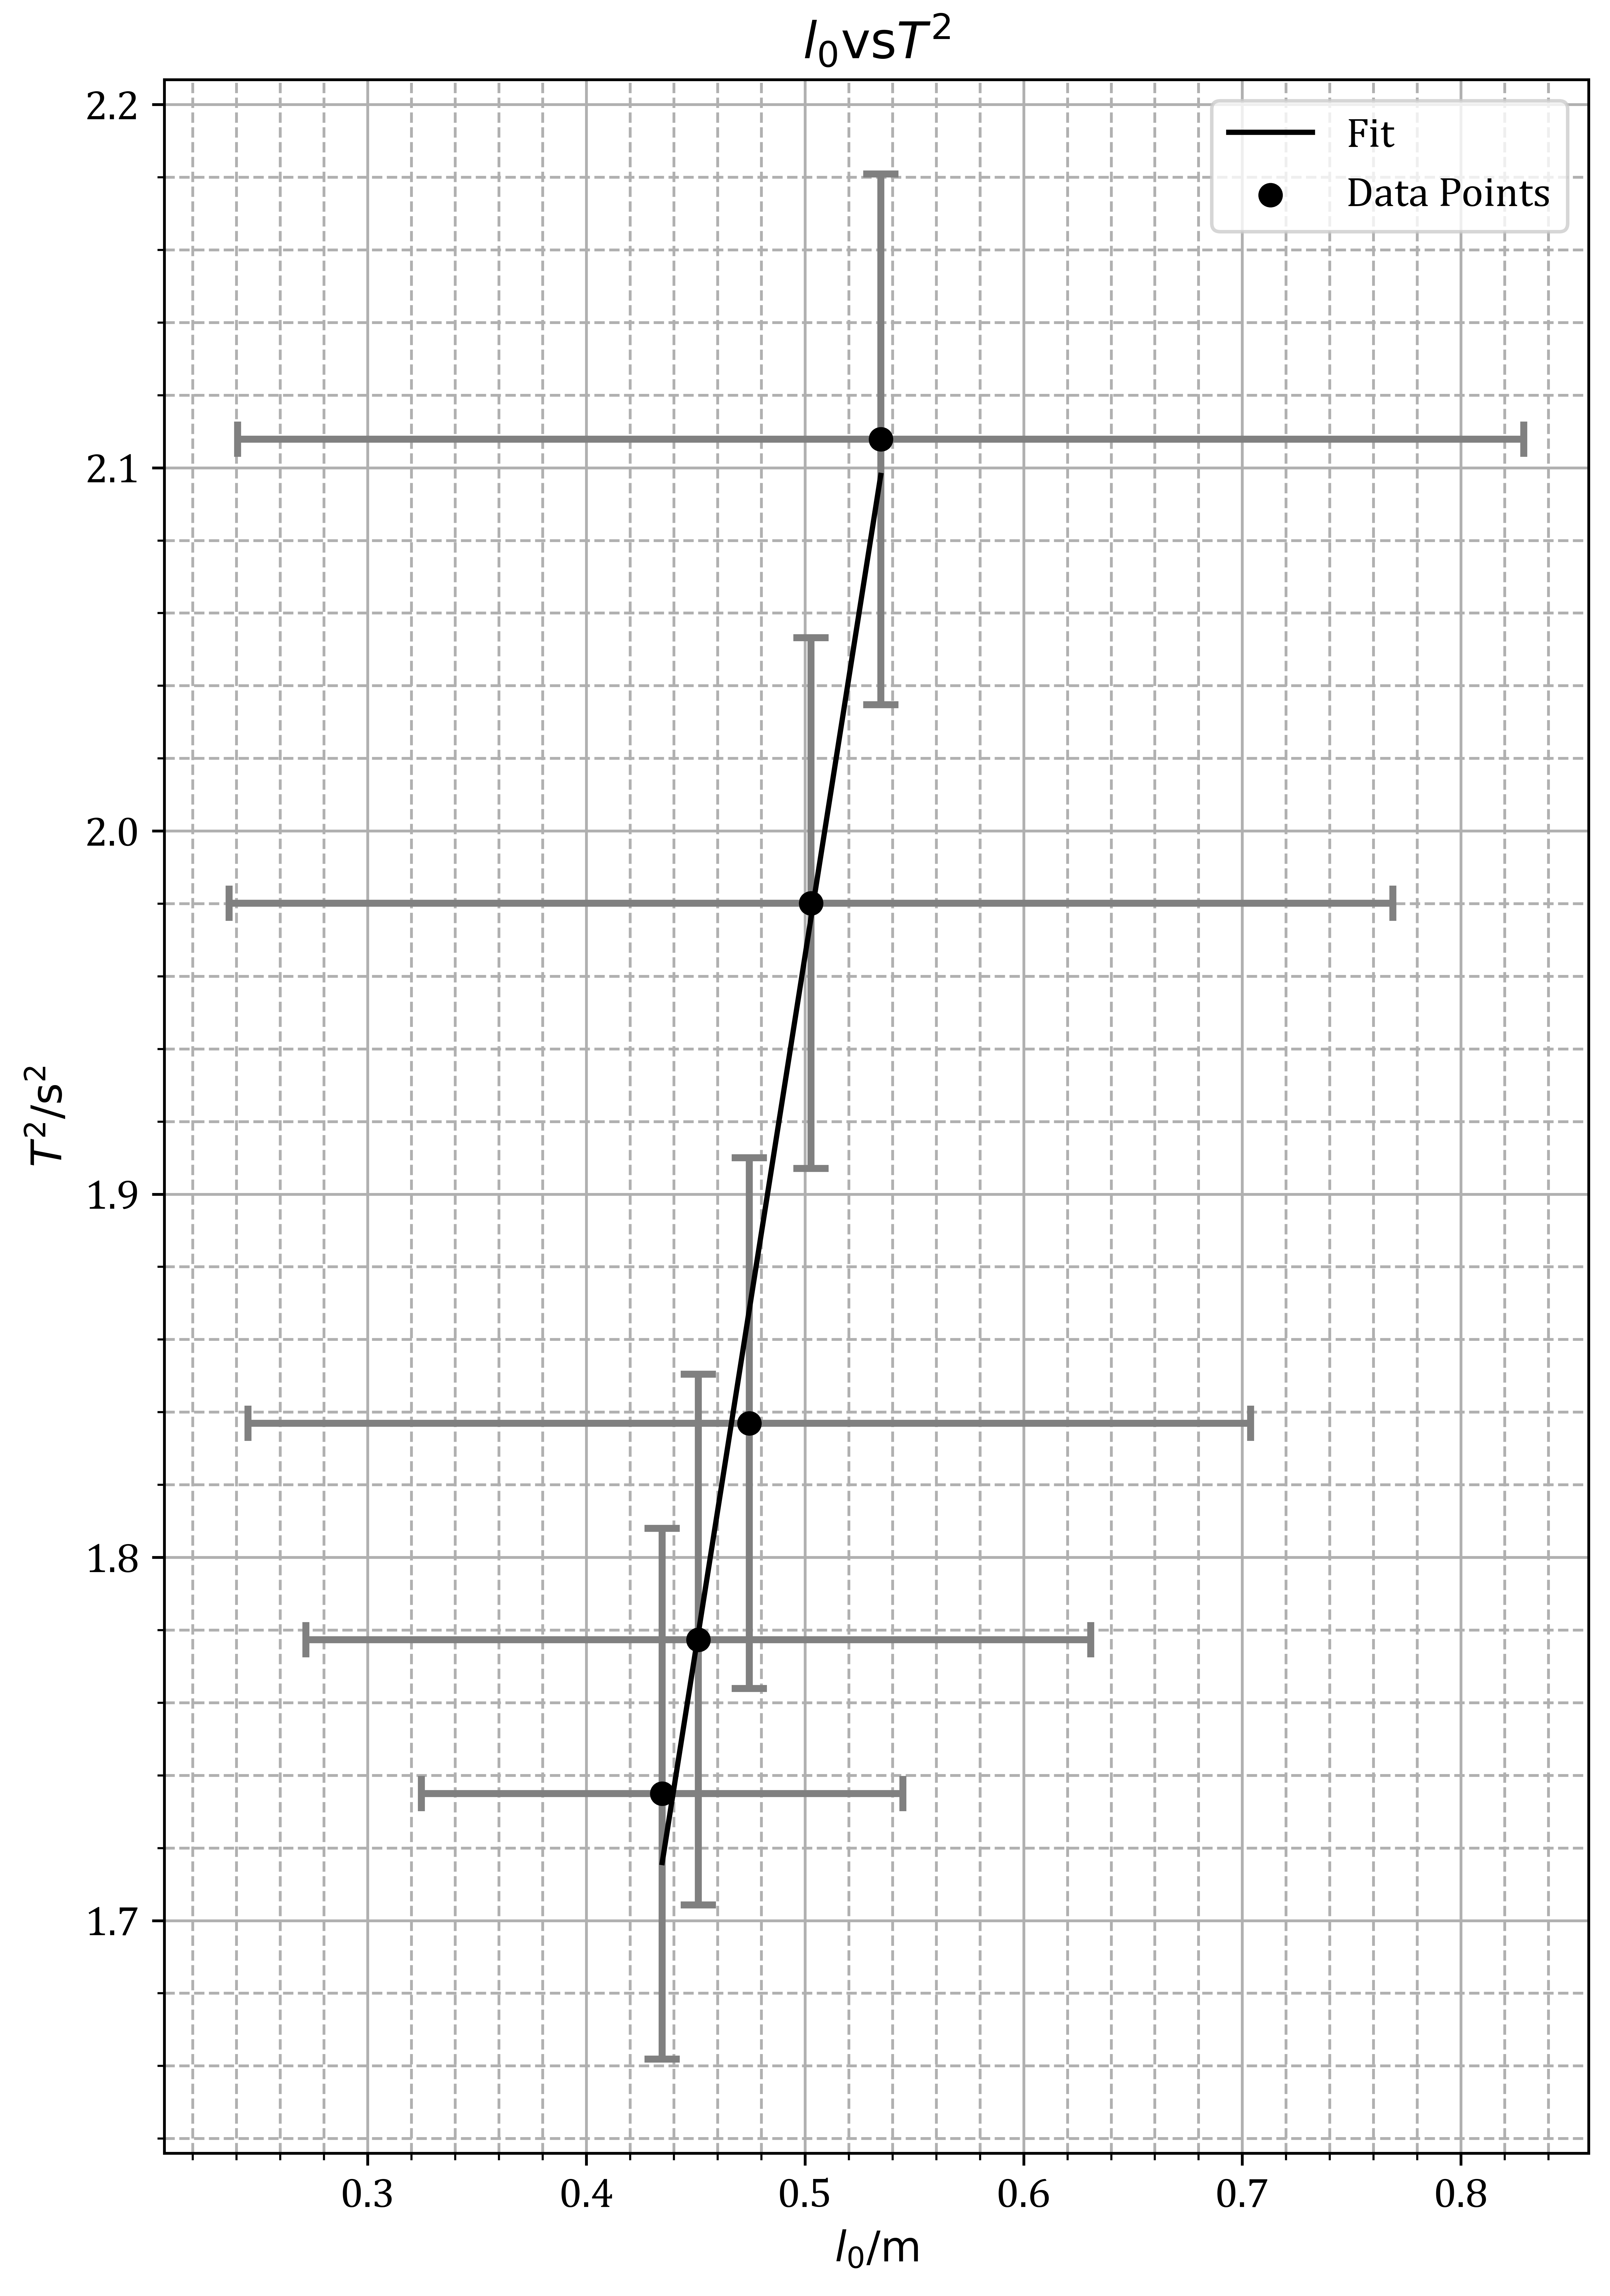
\includegraphics[width=\textwidth]{Gravgraph.png}
    \caption{$T^2 \text{ vs } l_0$}
    \label{fig:gravity graph}
\end{figure}

\section*{Calculations}
The data collected in the experiment was inputted into an excel sheet with the corresponding headers for the values, and it was read by the program using the following lines of code:
\begin{verbatim}
    data = pd.read_excel(`Experiment10Data.xlsx', 1)
    t2 = data[`T^2']
    l = data[`l']
    x_a = data[`x_averages']
    y_a = data[`y_averages']
\end{verbatim}
The averages of certain values, as the repeated values were stored in one column, were found using the following lines of code:
\begin{verbatim}
    L = data[`Lr'].mean()
    h = data[`h'].mean()
\end{verbatim}
Next, in order to obtain the mass ratio represented as $\frac{m}{M}$, the collected data for the $x$ and $y$ lengths was used in order to obtained a straight line graph using the following lines of code:
\begin{verbatim}
    coeffsm, covm = np.polyfit(x_a, y_a, 1, cov=True)
    poly_funcm = np.poly1d(coeffsm)
    trendlinem = poly_funcm(x_a)
\end{verbatim}
From this the mass ratio was found to $0.5934$ with an error of $0.0095$. The error for the gradient was found by square rooting the correct position of the co-variance matrix like so:
\begin{verbatim}
    deltaM = np.sqrt(covm[0][0]).
\end{verbatim}
In order to obtain the error values for the $x$ and $y$ lengths the following equation was used:
\begin{equation}\label{x,y error}
    \Delta x = t_{\alpha, n-1} \times \frac{s}{\sqrt{n}}
    \Delta y = t_{\alpha, n-1} \times \frac{s}{\sqrt{n}}
\end{equation}
where t is the t-value depending on the population in this case it was $4.30$, n is the population, and s is the standard deviation of the values. This was done through the use of the following lines of code:
\begin{verbatim}
    stdx = [np.std(data[`x1'].dropna(), axis=0, ddof=1), 
        np.std(data[`x2'].dropna(), axis=0, ddof=1),
        np.std(data[`x3'].dropna(), axis=0, ddof=1), 
        np.std(data[`x4'].dropna(), axis=0, ddof=1),
        np.std(data[`x5'].dropna(), axis=0, ddof=1)]
    deltax = tuple(map((4.30 / np.sqrt(3)).__mul__, stdx))
 
    stdy = [np.std(data[`y1'].dropna(), axis=0, ddof=1), 
        np.std(data[`y2'].dropna(), axis=0, ddof=1),
        np.std(data[`y3'].dropna(), axis=0, ddof=1), 
        np.std(data[`y4'].dropna(), axis=0, ddof=1),
        np.std(data[`y5'].dropna(), axis=0, ddof=1)]
    deltay = tuple(map((4.30 / np.sqrt(3)).__mul__, stdy)).
\end{verbatim}
After this $k$ was calculated using the following equation:
\begin{equation}\label{eqn: k equation}
    k = \frac{L}{\sqrt{12}}
\end{equation}
this was done through the use of code like so:
\begin{verbatim}
    k = L / np.sqrt(12).
\end{verbatim}
The average of h was then found and the standard deviation of them was calculated using these lines of code:
\begin{verbatim}
    h = data[`h'].mean()
    deltah = np.std([data[`h'].dropna()]) / data['h'].mean()
\end{verbatim}
These where then used in order to calculate the $l_0$ positions to be plotted against the $T^2$ positions. The $l_0$ positions were found using the following equation:
\begin{equation}\label{eqn: l0 equation}
    l_0 = \frac{\frac{m}{M}(h^2 + k^2) + l^2}{\frac{m}{M}h + l}
\end{equation}
This was done through the use of the following lines of code:
\begin{verbatim}
    def xplotfunction(x):
        return (M * ((h ** 2) + (k ** 2)) + (x ** 2)) / ((M * h) + x)
    xp = xplotfunction(l)
\end{verbatim}
where M is $\frac{m}{M}$ and x is then substituted for $l$. $T^2$ is found by first finding the average values of the time for 20 oscillations and then, dividing the values for different $l$ postions by 20. The answers to this were squared. These were then used in order to obtain the straight line graph equation needed to obtain the line of best fit for the data points. This was done using the following lines of code:
\begin{verbatim}
    coeffs, cov = np.polyfit(xp, t2, 1, cov=True)
    poly_func = np.poly1d(coeffs)
    trendline = poly_func(xp)
\end{verbatim}
The gradient of this straight line was found to be $3.0084$. The gradient in this case is equal to:
\begin{equation}\label{eqn: gradient g}
    \text{gradient} = \frac{4\pi}{g} 
\end{equation}
where g is the gravitational constant. This was then reformatted to obtain:
\begin{equation}\label{eqn: grav equation}
    g = \frac{4\pi ^2}{\text{gradient}}
\end{equation}
which results in the gravitational constant being equal to $10.3286\text{ ms}^{-2}$ with an error of $0.3701\text{ ms}^{-2}$, which was obtained through the following equation:
\begin{equation}\label{eqn: grav error}
    \Delta g = \frac{4\pi ^2}{\text{gradient}^2}
\end{equation}
In order to obtain the error bars for $T^2$ the standard deviation of the data set was calculated like so:
\begin{verbatim}
    deltat2 = np.std([data[`T^2'].dropna()]) / data['T^2'].mean()
\end{verbatim}
In order to calculate the combined error for the $l_0$ positions the following equation was used:
\begin{equation}\label{eqn: combined error}
    \partial l_0 = \sqrt{(\frac{\partial l_0}{\partial \frac{m}{M}}\times \Delta \frac{m}{M})^2 + (\frac{\partial l_0}{\partial h} \times \Delta h)^2 + (\frac{\partial l_0}{\partial k} \times \Delta k)^2 + (\frac{\partial l_0}{\partial l} \times \Delta l)^2}
\end{equation}
This was done through the use of the following lines of code:
\begin{verbatim}
    def derivative(e, f, g, p):
    a = Symbol(`a')
    b = Symbol(`b')
    c = Symbol(`c')
    d = Symbol(`d')
    equation = (a*(b ** 2 + c ** 2) + d ** 2) / (a * b + d)
    diff_a = Derivative(equation, a)
    diff_b = Derivative(equation, b)
    diff_c = Derivative(equation, c)
    diff_d = Derivative(equation, d)
    da = diff_a.doit()
    db = diff_b.doit()
    dc = diff_c.doit()
    dd = diff_d.doit()
    dM = da.subs({a: e, b: f, c: g, d: p}).evalf()
    dh = db.subs({a: e, b: f, c: g, d: p}).evalf()
    dk = dc.subs({a: e, b: f, c: g, d: p}).evalf()
    dl = dd.subs({a: e, b: f, c: g, d: p}).evalf()
    return ((np.power(dM, 2))*deltaM + (np.power(dh, 2))*deltah +     
            (np.power(dk, 2))*deltak + (np.power(dl, 2))*deltal)
            
    xerr = (sqrt(derivative(M, h, k, l[0])), 
            sqrt(derivative(M, h, k, l[1])), 
            sqrt(derivative(M, h, k, l[2])), 
            sqrt(derivative(M, h, k, l[3])), 
            sqrt(derivative(M, h, k, l[4])))
\end{verbatim}
where the initial variables of e, f, g, p are then replaced with the error values for $\frac{m}{M},\text{ }h,\text{ }k,\text{ }l$ respectively. This was done for each value of $l$. The accuracy of the gravitational constant was calculated as follows:
\begin{align*}
    \text{Accuracy} &= \frac{\text{Experimental Value}}{\text{Quoted value}}-1 \times 100\% \\
    &= \frac{10.3286}{9.81}-1 \times 100\% \\
    &= 5.29\%
\end{align*}
while the precision was calculated as follows:
\begin{align*}
    \text{Precision} &= \frac{\text{Combined error}}{\text{Experimental Value}} \times 100\% \\
    &= \frac{0.3701}{10.3286} \times 100\% \\
    &= 1.69\%
\end{align*}

\section*{Discussion}
The aim of this experiment was to find the gravitational constant without knowing the mass of both the rod and the mass being used, which required us to  first find the mass ratio $\frac{m}{M}$. The mass ration was found to be $0.5934\pm0.0095$ which was obtained from the gradient of figure \ref{fig:m/M graph}. With that value the $l_0$ for each value of $l$ was calculated with equation \ref{eqn: l0 equation}, which along with $T^2$ allowed us to obtain figure \ref{fig:gravity graph}. From the gradient of figure \ref{fig:gravity graph} and some reformatting, equation \ref{eqn: grav equation} was obtained and with the inputting of the values obtained, the gravitational constant was found to be $10.3286\pm0.3701 \text{ms}^{-2}$. These values had an accuracy of $5.29\%$ and a precision value of $1.75\%$. The low value of accuracy indicates that the results obtained from the experiment is close to the real value of the gravitational constant, but not completely accurate. This could be due to the fact that the pivot used to obtained the mass ratio was quite thick but not as thick as the minimum error of the meter ruler. The pivot used was not thin enough to be considered negligible, thus affecting the mass ratio. Also the open windows and students walking around the lab may have caused wind currents which may have caused the metal rod to gyrate slightly during the swinging, which would have affected the value of the time constant for each position of $l$. Furthermore, the parallax error encountered in the beginning of the experiment when taking the readings of $x$ and $y$ lengths will have affected the final value of the gravitational constant. However, the low value of precision indicated that even though the value obtained was slightly off from the real value, the readings were taken in a precise manner.

\smallskip
\noindent
Pendulums are not only used to keep track of time but rather they also have other uses in everyday life. Pendulums are used in seismometers, where the swinging of the pendulum is dictated by the earthquake happening which would allow for the location and calculating the strength of the earthquake taking place. The first recorded use of pendulums in such a way is accredited to Chinese scientist Zhange Heng \parencite{abel2019}. Another use of pendulums can be seen in playgrounds, where the swings used by children are a form of a pendulum. Furthermore pendulums were used by Kepler to determine the gravitational acceleration \parencite{taylor2019}. Robert Hooke had also used a variation of the normal pendulum called the conical pendulum to analyse the planet's orbit \parencite{taylor2019}.Additionally friction pendulums were created in order to protect buildings from earthquakes \parencite{abel2019}. These work by allowing the buildings to move side to side like a pendulum counter the movements of the earthquake, thus resulting in a reduction in building damage.

\printbibliography[title = {References:}]

\section*{Appendix}
\begin{verbatim}
import numpy as np
import pandas as pd
import matplotlib.pyplot as plt
from sympy import *
from math import sqrt
 
# importing data from excel sheet and defining variables
data = pd.read_excel(`Experiment10Data.xlsx', 1)
t2 = data[`T^2']
l = data[`l']
x_a = data[`x_averages']
y_a = data[`y_averages']
L = data[`Lr'].mean()
h = data[`h'].mean()
 
#finding the straight line equation of x vs y
coeffsm, covm = np.polyfit(x_a, y_a, 1, cov=True)
poly_funcm = np.poly1d(coeffsm)
trendlinem = poly_funcm(x_a)
 
#Finding the gradient and defining other variable
M = (coeffsm[0])
k = L / np.sqrt(12)
print(f`The mass ratio is {coeffsm[0]}')
 
# finding the error for the values of x and y for error bars
stdx = [np.std(data[`x1'].dropna(), axis=0, ddof=1), 
        np.std(data[`x2'].dropna(), axis=0, ddof=1),
        np.std(data[`x3'].dropna(), axis=0, ddof=1), 
        np.std(data[`x4'].dropna(), axis=0, ddof=1),
        np.std(data[`x5'].dropna(), axis=0, ddof=1)]
deltax = tuple(map((4.30 / np.sqrt(3)).__mul__, stdx))
 
stdy = [np.std(data[`y1'].dropna(), axis=0, ddof=1), 
        np.std(data[`y2'].dropna(), axis=0, ddof=1),
        np.std(data[`y3'].dropna(), axis=0, ddof=1), 
        np.std(data[`y4'].dropna(), axis=0, ddof=1),
        np.std(data[`y5'].dropna(), axis=0, ddof=1)]
deltay = tuple(map((4.30 / np.sqrt(3)).__mul__, stdy))
 
# finding error of m/M gradient
deltaM = np.sqrt(covm[0][0])
print(f`The error for m/M is {deltaM}')
 
# fiding error of other constants
deltah = np.std([data[`h'].dropna()]) / data['h'].mean()
deltak = np.std([data[`Lr'].dropna()]) / (data['Lr'].mean() * np.sqrt(12))
deltal = np.std([data[`l'].dropna()]) / data['l'].mean()
deltat2 = np.std([data[`T^2'].dropna()]) / data['T^2'].mean()
 
# defining the function for l_0
def xplotfunction(x):
    return (M * ((h ** 2) + (k ** 2)) + (x ** 2)) / ((M * h) + x)
 
# plugging in values for l to plot
xp = xplotfunction(l)
 
# defining a function for the partial derivation of l_0
def derivative(e, f, g, p):
    a = Symbol(`a')
    b = Symbol(`b')
    c = Symbol(`c')
    d = Symbol(`d')
    equation = (a*(b ** 2 + c ** 2) + d ** 2) / (a * b + d)
    diff_a = Derivative(equation, a)
    diff_b = Derivative(equation, b)
    diff_c = Derivative(equation, c)
    diff_d = Derivative(equation, d)
    da = diff_a.doit()
    db = diff_b.doit()
    dc = diff_c.doit()
    dd = diff_d.doit()
    dM = da.subs({a: e, b: f, c: g, d: p}).evalf()
    dh = db.subs({a: e, b: f, c: g, d: p}).evalf()
    dk = dc.subs({a: e, b: f, c: g, d: p}).evalf()
    dl = dd.subs({a: e, b: f, c: g, d: p}).evalf()
    return ((np.power(dM, 2))*deltaM + (np.power(dh, 2))*deltah +     
            (np.power(dk, 2))*deltak + (np.power(dl, 2))*deltal)
 
 
# calculating the combined error of l_0
xerr= (sqrt(derivative(M, h, k, l[0])), sqrt(derivative(M, h, k, l[1])), 
sqrt(derivative(M, h, k, l[2])), sqrt(derivative(M, h, k, l[3])), 
sqrt(derivative(M, h, k, l[4])))
 
# finding the straight line equation of T^2 vs l_0 and gradient
coeffs, cov = np.polyfit(xp, t2, 1, cov=True)
poly_func = np.poly1d(coeffs)
trendline = poly_func(xp)
print(f`The gradient of T^2 vs x is {coeffs[0]}')
 
# fidning gravity and its error
gravity = (4 * (np.pi ** 2)) / (coeffs[0])
print(f`Gravity is {gravity}')
deltagrav = (4 * np.pi ** 2) / gravity ** 2
print(f`The error of the gravity is {deltagrav}')
 
# defining the fonts and sizes to be used
plt.rcParams["font.family"] = "Cambria"
plt.rcParams["font.size"] = 12
plt.rcParams["font.weight"] = "normal"
 
f = plt.figure(figsize=(7.3, 10.7))
 
# plotting the error bars, data points, fitted line and axis, title are defined
plt.errorbar(x_a, y_a, xerr=deltax, yerr=deltay, fmt=`o', color=`k', elinewidth=2, 
            capthick=2, capsize=5, ecolor=`grey')
plt.scatter(x_a, y_a, color=`k', label=`Data Points')
plt.plot(x_a, trendlinem, color=`k', label=`Fit')
plt.minorticks_on()
plt.grid(b=True, which=`major', linestyle=`-')
plt.grid(b=True, which=`minor', linestyle=`--')
plt.legend()
plt.xlabel(r`$x \mathrm{/m}$')
plt.ylabel(r`$y \mathrm{/m}$')
plt.title(`x-distance vs y-distance')
plt.savefig(`mMgraph.png', dpi=800)
plt.show()

f = plt.figure(figsize=(7.3, 10.7))
 
# plotting the error bars, data points, fitted line and axis, title are defined
plt.errorbar(xp, t2, xerr=xerr, yerr=deltat2, fmt=`o', color=`k', elinewidth=2, 
            capthick=2, capsize=5, ecolor=`grey')
plt.scatter(xp, t2, color=`k', label=`Data Points')
plt.plot(xp, trendline, color=`k', label=`Fit')
plt.minorticks_on()
plt.grid(b=True, which=`major', linestyle=`-')
plt.grid(b=True, which=`minor', linestyle=`--')
plt.legend()
plt.xlabel(r`$l_0 \mathrm{/m}$')
plt.ylabel(r`$T^2 \mathrm{/s^2}$')
plt.title(r`$l_0 \mathrm{ vs } T^2$')
plt.savefig(`Gravgraph.png', dpi=800)
plt.show()
\end{verbatim}
\end{document}
